\begin{figure}[h]
  \centering
  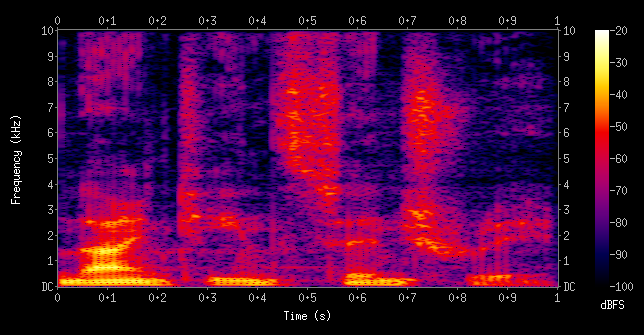
\includegraphics[width=12cm]{./Chapitre3/figures/spectrogramme.png}
  \caption{Représentation du signal en tant que spectogramme. La fréquence est modélisée en ordonnée et le temps en abscisse. L'énergie est visible grâce aux couleurs présentes: plus la couleur est chaude (rouge, orange, jaune) et plus l'énergie dégagée est importante. Image provenant de Wikipedia.}
  \label{fig:spectrogramme}
\end{figure}
